% Options for packages loaded elsewhere
\PassOptionsToPackage{unicode}{hyperref}
\PassOptionsToPackage{hyphens}{url}
%
\documentclass[
  ignorenonframetext,
]{beamer}
\usepackage{pgfpages}
\setbeamertemplate{caption}[numbered]
\setbeamertemplate{caption label separator}{: }
\setbeamercolor{caption name}{fg=normal text.fg}
\beamertemplatenavigationsymbolsempty
% Prevent slide breaks in the middle of a paragraph
\widowpenalties 1 10000
\raggedbottom
\setbeamertemplate{part page}{
  \centering
  \begin{beamercolorbox}[sep=16pt,center]{part title}
    \usebeamerfont{part title}\insertpart\par
  \end{beamercolorbox}
}
\setbeamertemplate{section page}{
  \centering
  \begin{beamercolorbox}[sep=12pt,center]{part title}
    \usebeamerfont{section title}\insertsection\par
  \end{beamercolorbox}
}
\setbeamertemplate{subsection page}{
  \centering
  \begin{beamercolorbox}[sep=8pt,center]{part title}
    \usebeamerfont{subsection title}\insertsubsection\par
  \end{beamercolorbox}
}
\AtBeginPart{
  \frame{\partpage}
}
\AtBeginSection{
  \ifbibliography
  \else
    \frame{\sectionpage}
  \fi
}
\AtBeginSubsection{
  \frame{\subsectionpage}
}
\usepackage{lmodern}
\usepackage{amssymb,amsmath}
\usepackage{ifxetex,ifluatex}
\ifnum 0\ifxetex 1\fi\ifluatex 1\fi=0 % if pdftex
  \usepackage[T1]{fontenc}
  \usepackage[utf8]{inputenc}
  \usepackage{textcomp} % provide euro and other symbols
\else % if luatex or xetex
  \usepackage{unicode-math}
  \defaultfontfeatures{Scale=MatchLowercase}
  \defaultfontfeatures[\rmfamily]{Ligatures=TeX,Scale=1}
\fi
% Use upquote if available, for straight quotes in verbatim environments
\IfFileExists{upquote.sty}{\usepackage{upquote}}{}
\IfFileExists{microtype.sty}{% use microtype if available
  \usepackage[]{microtype}
  \UseMicrotypeSet[protrusion]{basicmath} % disable protrusion for tt fonts
}{}
\makeatletter
\@ifundefined{KOMAClassName}{% if non-KOMA class
  \IfFileExists{parskip.sty}{%
    \usepackage{parskip}
  }{% else
    \setlength{\parindent}{0pt}
    \setlength{\parskip}{6pt plus 2pt minus 1pt}}
}{% if KOMA class
  \KOMAoptions{parskip=half}}
\makeatother
\usepackage{xcolor}
\IfFileExists{xurl.sty}{\usepackage{xurl}}{} % add URL line breaks if available
\IfFileExists{bookmark.sty}{\usepackage{bookmark}}{\usepackage{hyperref}}
\hypersetup{
  pdftitle={Module 9: Linear Regression},
  pdfauthor={Rebecca C. Steorts},
  hidelinks,
  pdfcreator={LaTeX via pandoc}}
\urlstyle{same} % disable monospaced font for URLs
\newif\ifbibliography
\usepackage{color}
\usepackage{fancyvrb}
\newcommand{\VerbBar}{|}
\newcommand{\VERB}{\Verb[commandchars=\\\{\}]}
\DefineVerbatimEnvironment{Highlighting}{Verbatim}{commandchars=\\\{\}}
% Add ',fontsize=\small' for more characters per line
\usepackage{framed}
\definecolor{shadecolor}{RGB}{248,248,248}
\newenvironment{Shaded}{\begin{snugshade}}{\end{snugshade}}
\newcommand{\AlertTok}[1]{\textcolor[rgb]{0.94,0.16,0.16}{#1}}
\newcommand{\AnnotationTok}[1]{\textcolor[rgb]{0.56,0.35,0.01}{\textbf{\textit{#1}}}}
\newcommand{\AttributeTok}[1]{\textcolor[rgb]{0.77,0.63,0.00}{#1}}
\newcommand{\BaseNTok}[1]{\textcolor[rgb]{0.00,0.00,0.81}{#1}}
\newcommand{\BuiltInTok}[1]{#1}
\newcommand{\CharTok}[1]{\textcolor[rgb]{0.31,0.60,0.02}{#1}}
\newcommand{\CommentTok}[1]{\textcolor[rgb]{0.56,0.35,0.01}{\textit{#1}}}
\newcommand{\CommentVarTok}[1]{\textcolor[rgb]{0.56,0.35,0.01}{\textbf{\textit{#1}}}}
\newcommand{\ConstantTok}[1]{\textcolor[rgb]{0.00,0.00,0.00}{#1}}
\newcommand{\ControlFlowTok}[1]{\textcolor[rgb]{0.13,0.29,0.53}{\textbf{#1}}}
\newcommand{\DataTypeTok}[1]{\textcolor[rgb]{0.13,0.29,0.53}{#1}}
\newcommand{\DecValTok}[1]{\textcolor[rgb]{0.00,0.00,0.81}{#1}}
\newcommand{\DocumentationTok}[1]{\textcolor[rgb]{0.56,0.35,0.01}{\textbf{\textit{#1}}}}
\newcommand{\ErrorTok}[1]{\textcolor[rgb]{0.64,0.00,0.00}{\textbf{#1}}}
\newcommand{\ExtensionTok}[1]{#1}
\newcommand{\FloatTok}[1]{\textcolor[rgb]{0.00,0.00,0.81}{#1}}
\newcommand{\FunctionTok}[1]{\textcolor[rgb]{0.00,0.00,0.00}{#1}}
\newcommand{\ImportTok}[1]{#1}
\newcommand{\InformationTok}[1]{\textcolor[rgb]{0.56,0.35,0.01}{\textbf{\textit{#1}}}}
\newcommand{\KeywordTok}[1]{\textcolor[rgb]{0.13,0.29,0.53}{\textbf{#1}}}
\newcommand{\NormalTok}[1]{#1}
\newcommand{\OperatorTok}[1]{\textcolor[rgb]{0.81,0.36,0.00}{\textbf{#1}}}
\newcommand{\OtherTok}[1]{\textcolor[rgb]{0.56,0.35,0.01}{#1}}
\newcommand{\PreprocessorTok}[1]{\textcolor[rgb]{0.56,0.35,0.01}{\textit{#1}}}
\newcommand{\RegionMarkerTok}[1]{#1}
\newcommand{\SpecialCharTok}[1]{\textcolor[rgb]{0.00,0.00,0.00}{#1}}
\newcommand{\SpecialStringTok}[1]{\textcolor[rgb]{0.31,0.60,0.02}{#1}}
\newcommand{\StringTok}[1]{\textcolor[rgb]{0.31,0.60,0.02}{#1}}
\newcommand{\VariableTok}[1]{\textcolor[rgb]{0.00,0.00,0.00}{#1}}
\newcommand{\VerbatimStringTok}[1]{\textcolor[rgb]{0.31,0.60,0.02}{#1}}
\newcommand{\WarningTok}[1]{\textcolor[rgb]{0.56,0.35,0.01}{\textbf{\textit{#1}}}}
\usepackage{graphicx,grffile}
\makeatletter
\def\maxwidth{\ifdim\Gin@nat@width>\linewidth\linewidth\else\Gin@nat@width\fi}
\def\maxheight{\ifdim\Gin@nat@height>\textheight\textheight\else\Gin@nat@height\fi}
\makeatother
% Scale images if necessary, so that they will not overflow the page
% margins by default, and it is still possible to overwrite the defaults
% using explicit options in \includegraphics[width, height, ...]{}
\setkeys{Gin}{width=\maxwidth,height=\maxheight,keepaspectratio}
% Set default figure placement to htbp
\makeatletter
\def\fps@figure{htbp}
\makeatother
\setlength{\emergencystretch}{3em} % prevent overfull lines
\providecommand{\tightlist}{%
  \setlength{\itemsep}{0pt}\setlength{\parskip}{0pt}}
\setcounter{secnumdepth}{-\maxdimen} % remove section numbering
% Custom definitions
% To use this customization file, insert the line "% Custom definitions
% To use this customization file, insert the line "% Custom definitions
% To use this customization file, insert the line "% Custom definitions
% To use this customization file, insert the line "\input{custom}" in the header of the tex file.

% Formatting

\tolerance=1000
\usepackage[margin=1in]{geometry}


% Packages

% \usepackage{amssymb,latexsym}
\usepackage{amssymb,amsfonts,amsmath,latexsym,amsthm}
\usepackage[usenames,dvipsnames]{color}
\usepackage[]{graphicx}
\usepackage[space]{grffile}
\usepackage{mathrsfs}   % fancy math font
% \usepackage[font=small,skip=0pt]{caption}
\usepackage[skip=0pt]{caption}
\usepackage{subcaption}
\usepackage{verbatim}
\usepackage{url}
\usepackage{bm}
\usepackage{dsfont}
\usepackage{extarrows}
\usepackage{multirow}
% \usepackage{wrapfig}
% \usepackage{epstopdf}
\usepackage{rotating}
\usepackage{tikz}
\usetikzlibrary{fit}					% fitting shapes to coordinates
%\usetikzlibrary{backgrounds}	% drawing the background after the foreground


% \usepackage[dvipdfm,colorlinks,citecolor=blue,linkcolor=blue,urlcolor=blue]{hyperref}
\usepackage[colorlinks,citecolor=blue,linkcolor=blue,urlcolor=blue]{hyperref}
%\usepackage{hyperref}
\usepackage[authoryear,round]{natbib}


%  Theorems, etc.

\theoremstyle{plain}
\newtheorem{theorem}{Theorem}[section]
\newtheorem{corollary}[theorem]{Corollary}
\newtheorem{lemma}[theorem]{Lemma}
\newtheorem{proposition}[theorem]{Proposition}
\newtheorem{condition}[theorem]{Condition}
% \newtheorem{conditions}[theorem]{Conditions}

\theoremstyle{definition}
\newtheorem{definition}[theorem]{Definition}
% \newtheorem*{unnumbered-definition}{Definition}
\newtheorem{example}[theorem]{Example}
\theoremstyle{remark}
\newtheorem*{remark}{Remark}
\numberwithin{equation}{section}




% Document-specific shortcuts
\newcommand{\btheta}{{\bm\theta}}
\newcommand{\bbtheta}{{\pmb{\bm\theta}}}

\newcommand{\commentary}[1]{\ifx\showcommentary\undefined\else \emph{#1}\fi}

\newcommand{\term}[1]{\textit{\textbf{#1}}}

% Math shortcuts

% Probability distributions
\DeclareMathOperator*{\Exp}{Exp}
\DeclareMathOperator*{\TExp}{TExp}
\DeclareMathOperator*{\Bernoulli}{Bernoulli}
\DeclareMathOperator*{\Beta}{Beta}
\DeclareMathOperator*{\Ga}{Gamma}
\DeclareMathOperator*{\TGamma}{TGamma}
\DeclareMathOperator*{\Poisson}{Poisson}
\DeclareMathOperator*{\Binomial}{Binomial}
\DeclareMathOperator*{\NormalGamma}{NormalGamma}
\DeclareMathOperator*{\InvGamma}{InvGamma}
\DeclareMathOperator*{\Cauchy}{Cauchy}
\DeclareMathOperator*{\Uniform}{Uniform}
\DeclareMathOperator*{\Gumbel}{Gumbel}
\DeclareMathOperator*{\Pareto}{Pareto}
\DeclareMathOperator*{\Mono}{Mono}
\DeclareMathOperator*{\Geometric}{Geometric}
\DeclareMathOperator*{\Wishart}{Wishart}

% Math operators
\DeclareMathOperator*{\argmin}{arg\,min}
\DeclareMathOperator*{\argmax}{arg\,max}
\DeclareMathOperator*{\Cov}{Cov}
\DeclareMathOperator*{\diag}{diag}
\DeclareMathOperator*{\median}{median}
\DeclareMathOperator*{\Vol}{Vol}

% Math characters
\newcommand{\R}{\mathbb{R}}
\newcommand{\Z}{\mathbb{Z}}
\newcommand{\E}{\mathbb{E}}
\renewcommand{\Pr}{\mathbb{P}}
\newcommand{\I}{\mathds{1}}
\newcommand{\V}{\mathbb{V}}

\newcommand{\A}{\mathcal{A}}
\newcommand{\C}{\mathcal{C}}
\newcommand{\D}{\mathcal{D}}
\newcommand{\Hcal}{\mathcal{H}}
\newcommand{\M}{\mathcal{M}}
\newcommand{\N}{\mathcal{N}}
\newcommand{\X}{\mathcal{X}}
\newcommand{\Zcal}{\mathcal{Z}}
\renewcommand{\P}{\mathcal{P}}

\newcommand{\T}{\mathtt{T}}
\renewcommand{\emptyset}{\varnothing}


% Miscellaneous commands
\newcommand{\iid}{\stackrel{\mathrm{iid}}{\sim}}
\newcommand{\matrixsmall}[1]{\bigl(\begin{smallmatrix}#1\end{smallmatrix} \bigr)}

\newcommand{\items}[1]{\begin{itemize} #1 \end{itemize}}

\newcommand{\todo}[1]{\emph{\textcolor{red}{(#1)}}}

\newcommand{\branch}[4]{
\left\{
	\begin{array}{ll}
		#1  & \mbox{if } #2 \\
		#3 & \mbox{if } #4
	\end{array}
\right.
}

% approximately proportional to
\def\app#1#2{%
  \mathrel{%
    \setbox0=\hbox{$#1\sim$}%
    \setbox2=\hbox{%
      \rlap{\hbox{$#1\propto$}}%
      \lower1.3\ht0\box0%
    }%
    \raise0.25\ht2\box2%
  }%
}
\def\approxprop{\mathpalette\app\relax}

% \newcommand{\approptoinn}[2]{\mathrel{\vcenter{
  % \offinterlineskip\halign{\hfil$##$\cr
    % #1\propto\cr\noalign{\kern2pt}#1\sim\cr\noalign{\kern-2pt}}}}}

% \newcommand{\approxpropto}{\mathpalette\approptoinn\relax}





" in the header of the tex file.

% Formatting

\tolerance=1000
\usepackage[margin=1in]{geometry}


% Packages

% \usepackage{amssymb,latexsym}
\usepackage{amssymb,amsfonts,amsmath,latexsym,amsthm}
\usepackage[usenames,dvipsnames]{color}
\usepackage[]{graphicx}
\usepackage[space]{grffile}
\usepackage{mathrsfs}   % fancy math font
% \usepackage[font=small,skip=0pt]{caption}
\usepackage[skip=0pt]{caption}
\usepackage{subcaption}
\usepackage{verbatim}
\usepackage{url}
\usepackage{bm}
\usepackage{dsfont}
\usepackage{extarrows}
\usepackage{multirow}
% \usepackage{wrapfig}
% \usepackage{epstopdf}
\usepackage{rotating}
\usepackage{tikz}
\usetikzlibrary{fit}					% fitting shapes to coordinates
%\usetikzlibrary{backgrounds}	% drawing the background after the foreground


% \usepackage[dvipdfm,colorlinks,citecolor=blue,linkcolor=blue,urlcolor=blue]{hyperref}
\usepackage[colorlinks,citecolor=blue,linkcolor=blue,urlcolor=blue]{hyperref}
%\usepackage{hyperref}
\usepackage[authoryear,round]{natbib}


%  Theorems, etc.

\theoremstyle{plain}
\newtheorem{theorem}{Theorem}[section]
\newtheorem{corollary}[theorem]{Corollary}
\newtheorem{lemma}[theorem]{Lemma}
\newtheorem{proposition}[theorem]{Proposition}
\newtheorem{condition}[theorem]{Condition}
% \newtheorem{conditions}[theorem]{Conditions}

\theoremstyle{definition}
\newtheorem{definition}[theorem]{Definition}
% \newtheorem*{unnumbered-definition}{Definition}
\newtheorem{example}[theorem]{Example}
\theoremstyle{remark}
\newtheorem*{remark}{Remark}
\numberwithin{equation}{section}




% Document-specific shortcuts
\newcommand{\btheta}{{\bm\theta}}
\newcommand{\bbtheta}{{\pmb{\bm\theta}}}

\newcommand{\commentary}[1]{\ifx\showcommentary\undefined\else \emph{#1}\fi}

\newcommand{\term}[1]{\textit{\textbf{#1}}}

% Math shortcuts

% Probability distributions
\DeclareMathOperator*{\Exp}{Exp}
\DeclareMathOperator*{\TExp}{TExp}
\DeclareMathOperator*{\Bernoulli}{Bernoulli}
\DeclareMathOperator*{\Beta}{Beta}
\DeclareMathOperator*{\Ga}{Gamma}
\DeclareMathOperator*{\TGamma}{TGamma}
\DeclareMathOperator*{\Poisson}{Poisson}
\DeclareMathOperator*{\Binomial}{Binomial}
\DeclareMathOperator*{\NormalGamma}{NormalGamma}
\DeclareMathOperator*{\InvGamma}{InvGamma}
\DeclareMathOperator*{\Cauchy}{Cauchy}
\DeclareMathOperator*{\Uniform}{Uniform}
\DeclareMathOperator*{\Gumbel}{Gumbel}
\DeclareMathOperator*{\Pareto}{Pareto}
\DeclareMathOperator*{\Mono}{Mono}
\DeclareMathOperator*{\Geometric}{Geometric}
\DeclareMathOperator*{\Wishart}{Wishart}

% Math operators
\DeclareMathOperator*{\argmin}{arg\,min}
\DeclareMathOperator*{\argmax}{arg\,max}
\DeclareMathOperator*{\Cov}{Cov}
\DeclareMathOperator*{\diag}{diag}
\DeclareMathOperator*{\median}{median}
\DeclareMathOperator*{\Vol}{Vol}

% Math characters
\newcommand{\R}{\mathbb{R}}
\newcommand{\Z}{\mathbb{Z}}
\newcommand{\E}{\mathbb{E}}
\renewcommand{\Pr}{\mathbb{P}}
\newcommand{\I}{\mathds{1}}
\newcommand{\V}{\mathbb{V}}

\newcommand{\A}{\mathcal{A}}
\newcommand{\C}{\mathcal{C}}
\newcommand{\D}{\mathcal{D}}
\newcommand{\Hcal}{\mathcal{H}}
\newcommand{\M}{\mathcal{M}}
\newcommand{\N}{\mathcal{N}}
\newcommand{\X}{\mathcal{X}}
\newcommand{\Zcal}{\mathcal{Z}}
\renewcommand{\P}{\mathcal{P}}

\newcommand{\T}{\mathtt{T}}
\renewcommand{\emptyset}{\varnothing}


% Miscellaneous commands
\newcommand{\iid}{\stackrel{\mathrm{iid}}{\sim}}
\newcommand{\matrixsmall}[1]{\bigl(\begin{smallmatrix}#1\end{smallmatrix} \bigr)}

\newcommand{\items}[1]{\begin{itemize} #1 \end{itemize}}

\newcommand{\todo}[1]{\emph{\textcolor{red}{(#1)}}}

\newcommand{\branch}[4]{
\left\{
	\begin{array}{ll}
		#1  & \mbox{if } #2 \\
		#3 & \mbox{if } #4
	\end{array}
\right.
}

% approximately proportional to
\def\app#1#2{%
  \mathrel{%
    \setbox0=\hbox{$#1\sim$}%
    \setbox2=\hbox{%
      \rlap{\hbox{$#1\propto$}}%
      \lower1.3\ht0\box0%
    }%
    \raise0.25\ht2\box2%
  }%
}
\def\approxprop{\mathpalette\app\relax}

% \newcommand{\approptoinn}[2]{\mathrel{\vcenter{
  % \offinterlineskip\halign{\hfil$##$\cr
    % #1\propto\cr\noalign{\kern2pt}#1\sim\cr\noalign{\kern-2pt}}}}}

% \newcommand{\approxpropto}{\mathpalette\approptoinn\relax}





" in the header of the tex file.

% Formatting

\tolerance=1000
\usepackage[margin=1in]{geometry}


% Packages

% \usepackage{amssymb,latexsym}
\usepackage{amssymb,amsfonts,amsmath,latexsym,amsthm}
\usepackage[usenames,dvipsnames]{color}
\usepackage[]{graphicx}
\usepackage[space]{grffile}
\usepackage{mathrsfs}   % fancy math font
% \usepackage[font=small,skip=0pt]{caption}
\usepackage[skip=0pt]{caption}
\usepackage{subcaption}
\usepackage{verbatim}
\usepackage{url}
\usepackage{bm}
\usepackage{dsfont}
\usepackage{extarrows}
\usepackage{multirow}
% \usepackage{wrapfig}
% \usepackage{epstopdf}
\usepackage{rotating}
\usepackage{tikz}
\usetikzlibrary{fit}					% fitting shapes to coordinates
%\usetikzlibrary{backgrounds}	% drawing the background after the foreground


% \usepackage[dvipdfm,colorlinks,citecolor=blue,linkcolor=blue,urlcolor=blue]{hyperref}
\usepackage[colorlinks,citecolor=blue,linkcolor=blue,urlcolor=blue]{hyperref}
%\usepackage{hyperref}
\usepackage[authoryear,round]{natbib}


%  Theorems, etc.

\theoremstyle{plain}
\newtheorem{theorem}{Theorem}[section]
\newtheorem{corollary}[theorem]{Corollary}
\newtheorem{lemma}[theorem]{Lemma}
\newtheorem{proposition}[theorem]{Proposition}
\newtheorem{condition}[theorem]{Condition}
% \newtheorem{conditions}[theorem]{Conditions}

\theoremstyle{definition}
\newtheorem{definition}[theorem]{Definition}
% \newtheorem*{unnumbered-definition}{Definition}
\newtheorem{example}[theorem]{Example}
\theoremstyle{remark}
\newtheorem*{remark}{Remark}
\numberwithin{equation}{section}




% Document-specific shortcuts
\newcommand{\btheta}{{\bm\theta}}
\newcommand{\bbtheta}{{\pmb{\bm\theta}}}

\newcommand{\commentary}[1]{\ifx\showcommentary\undefined\else \emph{#1}\fi}

\newcommand{\term}[1]{\textit{\textbf{#1}}}

% Math shortcuts

% Probability distributions
\DeclareMathOperator*{\Exp}{Exp}
\DeclareMathOperator*{\TExp}{TExp}
\DeclareMathOperator*{\Bernoulli}{Bernoulli}
\DeclareMathOperator*{\Beta}{Beta}
\DeclareMathOperator*{\Ga}{Gamma}
\DeclareMathOperator*{\TGamma}{TGamma}
\DeclareMathOperator*{\Poisson}{Poisson}
\DeclareMathOperator*{\Binomial}{Binomial}
\DeclareMathOperator*{\NormalGamma}{NormalGamma}
\DeclareMathOperator*{\InvGamma}{InvGamma}
\DeclareMathOperator*{\Cauchy}{Cauchy}
\DeclareMathOperator*{\Uniform}{Uniform}
\DeclareMathOperator*{\Gumbel}{Gumbel}
\DeclareMathOperator*{\Pareto}{Pareto}
\DeclareMathOperator*{\Mono}{Mono}
\DeclareMathOperator*{\Geometric}{Geometric}
\DeclareMathOperator*{\Wishart}{Wishart}

% Math operators
\DeclareMathOperator*{\argmin}{arg\,min}
\DeclareMathOperator*{\argmax}{arg\,max}
\DeclareMathOperator*{\Cov}{Cov}
\DeclareMathOperator*{\diag}{diag}
\DeclareMathOperator*{\median}{median}
\DeclareMathOperator*{\Vol}{Vol}

% Math characters
\newcommand{\R}{\mathbb{R}}
\newcommand{\Z}{\mathbb{Z}}
\newcommand{\E}{\mathbb{E}}
\renewcommand{\Pr}{\mathbb{P}}
\newcommand{\I}{\mathds{1}}
\newcommand{\V}{\mathbb{V}}

\newcommand{\A}{\mathcal{A}}
\newcommand{\C}{\mathcal{C}}
\newcommand{\D}{\mathcal{D}}
\newcommand{\Hcal}{\mathcal{H}}
\newcommand{\M}{\mathcal{M}}
\newcommand{\N}{\mathcal{N}}
\newcommand{\X}{\mathcal{X}}
\newcommand{\Zcal}{\mathcal{Z}}
\renewcommand{\P}{\mathcal{P}}

\newcommand{\T}{\mathtt{T}}
\renewcommand{\emptyset}{\varnothing}


% Miscellaneous commands
\newcommand{\iid}{\stackrel{\mathrm{iid}}{\sim}}
\newcommand{\matrixsmall}[1]{\bigl(\begin{smallmatrix}#1\end{smallmatrix} \bigr)}

\newcommand{\items}[1]{\begin{itemize} #1 \end{itemize}}

\newcommand{\todo}[1]{\emph{\textcolor{red}{(#1)}}}

\newcommand{\branch}[4]{
\left\{
	\begin{array}{ll}
		#1  & \mbox{if } #2 \\
		#3 & \mbox{if } #4
	\end{array}
\right.
}

% approximately proportional to
\def\app#1#2{%
  \mathrel{%
    \setbox0=\hbox{$#1\sim$}%
    \setbox2=\hbox{%
      \rlap{\hbox{$#1\propto$}}%
      \lower1.3\ht0\box0%
    }%
    \raise0.25\ht2\box2%
  }%
}
\def\approxprop{\mathpalette\app\relax}

% \newcommand{\approptoinn}[2]{\mathrel{\vcenter{
  % \offinterlineskip\halign{\hfil$##$\cr
    % #1\propto\cr\noalign{\kern2pt}#1\sim\cr\noalign{\kern-2pt}}}}}

% \newcommand{\approxpropto}{\mathpalette\approptoinn\relax}





" in the header of the tex file.

% Formatting

\setbeamertemplate{navigation symbols}{}
\setbeamertemplate{footline}[page number]

\usepackage{bbm}
% Packages
\usepackage{amssymb,amsfonts,amsmath,latexsym,amsthm}
%\usepackage[usenames,dvipsnames]{color}
%\usepackage[]{graphicx}
%\usepackage[space]{grffile}
\usepackage{mathrsfs} 
 \usepackage{amssymb,latexsym}
\usepackage{amssymb,amsfonts,amsmath,latexsym,amsthm, bm}
%\usepackage[usenames,dvipsnames]{color}
%\usepackage[]{graphicx}
%\usepackage[space]{grffile}
\usepackage{mathrsfs}   % fancy math font
% \usepackage[font=small,skip=0pt]{caption}
%\usepackage[skip=0pt]{caption}
%\usepackage{subcaption}
%\usepackage{verbatim}
%\usepackage{url}
%\usepackage{bm}
\usepackage{dsfont}
\usepackage{multirow}
%\usepackage{extarrows}
%\usepackage{multirow}
%% \usepackage{wrapfig}
%% \usepackage{epstopdf}
%\usepackage{rotating}
%\usepackage{tikz}
%\usetikzlibrary{fit}					% fitting shapes to coordinates
%\usetikzlibrary{backgrounds}	% drawing the background after the foreground


% \usepackage[dvipdfm,colorlinks,citecolor=blue,linkcolor=blue,urlcolor=blue]{hyperref}
%\usepackage[colorlinks,citecolor=blue,linkcolor=blue,urlcolor=blue]{hyperref}
%%\usepackage{hyperref}
%\usepackage[authoryear,round]{natbib}


%  Theorems, etc.

%\theoremstyle{plain}
%\newtheorem{theorem}{Theorem}[section]
%\newtheorem{corollary}[theorem]{Corollary}
%\newtheorem{lemma}[theorem]{Lemma}
%\newtheorem{proposition}[theorem]{Proposition}
%\newtheorem{condition}[theorem]{Condition}
% \newtheorem{conditions}[theorem]{Conditions}

%\theoremstyle{definition}
%\newtheorem{definition}[theorem]{Definition}
%% \newtheorem*{unnumbered-definition}{Definition}
%\newtheorem{example}[theorem]{Example}
%\theoremstyle{remark}
%\newtheorem*{remark}{Remark}
%\numberwithin{equation}{section}

\newcommand{\bx}   {\bm{x}}
\newcommand{\bY}   {\bm{Y}}
\newcommand{\by}   {\bm{y}}

\newcommand{\hbeta}   {\hat{\beta}}
\newcommand{\hy}   {\hat{y}}


% Document-specific shortcuts
\newcommand{\btheta}{{\bm\theta}}
\newcommand{\bbtheta}{{\pmb{\bm\theta}}}

\newcommand{\commentary}[1]{\ifx\showcommentary\undefined\else \emph{#1}\fi}

\newcommand{\term}[1]{\textit{\textbf{#1}}}

% Math shortcuts

% Probability distributions
\DeclareMathOperator*{\Exp}{Exp}
\DeclareMathOperator*{\TExp}{TExp}
\DeclareMathOperator*{\Bernoulli}{Bernoulli}
\DeclareMathOperator*{\Beta}{Beta}
\DeclareMathOperator*{\Ga}{Gamma}
\DeclareMathOperator*{\TGamma}{TGamma}
\DeclareMathOperator*{\Poisson}{Poisson}
\DeclareMathOperator*{\Binomial}{Binomial}
\DeclareMathOperator*{\NormalGamma}{NormalGamma}
\DeclareMathOperator*{\InvGamma}{InvGamma}
\DeclareMathOperator*{\Cauchy}{Cauchy}
\DeclareMathOperator*{\Uniform}{Uniform}
\DeclareMathOperator*{\Gumbel}{Gumbel}
\DeclareMathOperator*{\Pareto}{Pareto}
\DeclareMathOperator*{\Mono}{Mono}
\DeclareMathOperator*{\Geometric}{Geometric}
\DeclareMathOperator*{\Wishart}{Wishart}

% Math operators
\DeclareMathOperator*{\argmin}{arg\,min}
\DeclareMathOperator*{\argmax}{arg\,max}
\DeclareMathOperator*{\Cov}{Cov}
\DeclareMathOperator*{\diag}{diag}
\DeclareMathOperator*{\median}{median}
\DeclareMathOperator*{\Vol}{Vol}

% Math characters
\newcommand{\R}{\mathbb{R}}
\newcommand{\Z}{\mathbb{Z}}
\newcommand{\E}{\mathbb{E}}
\renewcommand{\Pr}{\mathbb{P}}
\newcommand{\I}{\mathds{1}}
\newcommand{\V}{\mathbb{V}}
\newcommand{\bbeta}{\bm{\beta}}

\newcommand{\A}{\mathcal{A}}
%\newcommand{\C}{\mathcal{C}}
\newcommand{\D}{\mathcal{D}}
\newcommand{\Hcal}{\mathcal{H}}
\newcommand{\M}{\mathcal{M}}
\newcommand{\N}{\mathcal{N}}
\newcommand{\X}{\mathcal{X}}
\newcommand{\Zcal}{\mathcal{Z}}
\renewcommand{\P}{\mathcal{P}}


\newcommand{\T}{\mathtt{T}}
\renewcommand{\emptyset}{\varnothing}

\newcommand{\bmu}{\bm{\mu}}
\newcommand{\bX}   {\bm{X}}
\newcommand{\sig}   {\Sigma}
%\newcommand{\X}{\ensuremath{\mathbf{x}}}
%\newcommand{\w}{\ensuremath{\mathbf{w}}}
%\newcommand{\h}{\ensuremath{\mathbf{h}}}
%\newcommand{\V}{\ensuremath{\mathbf{v}}}
%\newcommand{\cov}{\text{Cov}}
\newcommand{\var}{\text{Var}}
\newcommand{\Var}{\text{Var}}



% Miscellaneous commands
\newcommand{\iid}{\stackrel{\mathrm{iid}}{\sim}}
\newcommand{\matrixsmall}[1]{\bigl(\begin{smallmatrix}#1\end{smallmatrix} \bigr)}

\newcommand{\items}[1]{\begin{itemize} #1 \end{itemize}}

\newcommand{\todo}[1]{\emph{\textcolor{red}{(#1)}}}

\newcommand{\branch}[4]{
\left\{
	\begin{array}{ll}
		#1  & \mbox{if } #2 \\
		#3 & \mbox{if } #4
	\end{array}
\right.
}

% approximately proportional to
\def\app#1#2{%
  \mathrel{%
    \setbox0=\hbox{$#1\sim$}%
    \setbox2=\hbox{%
      \rlap{\hbox{$#1\propto$}}%
      \lower1.3\ht0\box0%
    }%
    \raise0.25\ht2\box2%
  }%
}
\def\approxprop{\mathpalette\app\relax}

% \newcommand{\approptoinn}[2]{\mathrel{\vcenter{
  % \offinterlineskip\halign{\hfil$##$\cr
    % #1\propto\cr\noalign{\kern2pt}#1\sim\cr\noalign{\kern-2pt}}}}}

% \newcommand{\approxpropto}{\mathpalette\approptoinn\relax}

\title{Module 9: Linear Regression}
\author{Rebecca C. Steorts}
\date{Hoff, Chapter 9}

\begin{document}
\frame{\titlepage}

\begin{frame}{Remainder of Semester}
\protect\hypertarget{remainder-of-semester}{}

\textbf{This week}

\begin{itemize}
\tightlist
\item
  Thursday, November 5: Linear Regression
\item
  Friday, November 6: Lab 10 (Homework 8)
\end{itemize}

\vspace*{1em}

\textbf{Next week}

\begin{itemize}
\tightlist
\item
  Tuesday, November 10: Linear and Logistic Regression
\item
  Thursday, November 12: Logistic Regression + Final Exam
\item
  Friday November 13, 5 PM EDT: Homework 8 (last homework + extra
  credit)
\end{itemize}

\vspace*{1em}

\textbf{Reading period}

\begin{itemize}
\tightlist
\item
  All OH will be held. Mine will be during class to avoid any conflicts
  and be more friendly to international students.
\end{itemize}

\end{frame}

\begin{frame}{Final Exam}
\protect\hypertarget{final-exam}{}

The final exam is \textbf{November 22, 2 PM - 5 PM EDT} (open note/open
book)

\begin{itemize}
\tightlist
\item
  The material will be on modules 1 -- 9.
\item
  I will go over more details regarding the exam next week
\end{itemize}

\end{frame}

\begin{frame}{Agenda}
\protect\hypertarget{agenda}{}

\begin{itemize}
\tightlist
\item
  Motivation: oxygen uptake example
\item
  Linear regression
\item
  Multiple and Multivariate Linear Regression
\item
  Bayesian Linear Regression
\item
  Background on the Euclidean norm and argmin
\item
  Ordinary Least Squares + Exercises
\item
  Setting Prior Parameters
\item
  The g-prior
\item
  How does this all fit together
\end{itemize}

\end{frame}

\begin{frame}{Oxygen uptake case study}
\protect\hypertarget{oxygen-uptake-case-study}{}

Experimental design: 12 male volunteers.

\begin{enumerate}
\item $O_2$ uptake measured at the beginning of the study
\item 6 men take part in a randomized aerobics program
\item 6 remaining men participate in a running program
\item $O_2$ uptake measured at end of study
\end{enumerate}

What type of exercise is the most beneficial?

\end{frame}

\begin{frame}[fragile]{Data}
\protect\hypertarget{data}{}

\begin{Shaded}
\begin{Highlighting}[]
\CommentTok{# 0 is running}
\CommentTok{# 1 is aerobic exercise}
\NormalTok{x1<-}\KeywordTok{c}\NormalTok{(}\DecValTok{0}\NormalTok{,}\DecValTok{0}\NormalTok{,}\DecValTok{0}\NormalTok{,}\DecValTok{0}\NormalTok{,}\DecValTok{0}\NormalTok{,}\DecValTok{0}\NormalTok{,}\DecValTok{1}\NormalTok{,}\DecValTok{1}\NormalTok{,}\DecValTok{1}\NormalTok{,}\DecValTok{1}\NormalTok{,}\DecValTok{1}\NormalTok{,}\DecValTok{1}\NormalTok{)}
\CommentTok{# x2 is age}
\NormalTok{x2<-}\KeywordTok{c}\NormalTok{(}\DecValTok{23}\NormalTok{,}\DecValTok{22}\NormalTok{,}\DecValTok{22}\NormalTok{,}\DecValTok{25}\NormalTok{,}\DecValTok{27}\NormalTok{,}\DecValTok{20}\NormalTok{,}\DecValTok{31}\NormalTok{,}\DecValTok{23}\NormalTok{,}\DecValTok{27}\NormalTok{,}\DecValTok{28}\NormalTok{,}\DecValTok{22}\NormalTok{,}\DecValTok{24}\NormalTok{)}
\CommentTok{# change in maximal oxygen uptake}
\NormalTok{y<-}\KeywordTok{c}\NormalTok{(}\OperatorTok{-}\FloatTok{0.87}\NormalTok{,}\OperatorTok{-}\FloatTok{10.74}\NormalTok{,}\OperatorTok{-}\FloatTok{3.27}\NormalTok{,}\OperatorTok{-}\FloatTok{1.97}\NormalTok{,}\FloatTok{7.50}\NormalTok{,}
     \FloatTok{-7.25}\NormalTok{,}\FloatTok{17.05}\NormalTok{,}\FloatTok{4.96}\NormalTok{,}\FloatTok{10.40}\NormalTok{,}\FloatTok{11.05}\NormalTok{,}\FloatTok{0.26}\NormalTok{,}\FloatTok{2.51}\NormalTok{)}
\end{Highlighting}
\end{Shaded}

\end{frame}

\begin{frame}{Exploratory Data Analysis}
\protect\hypertarget{exploratory-data-analysis}{}

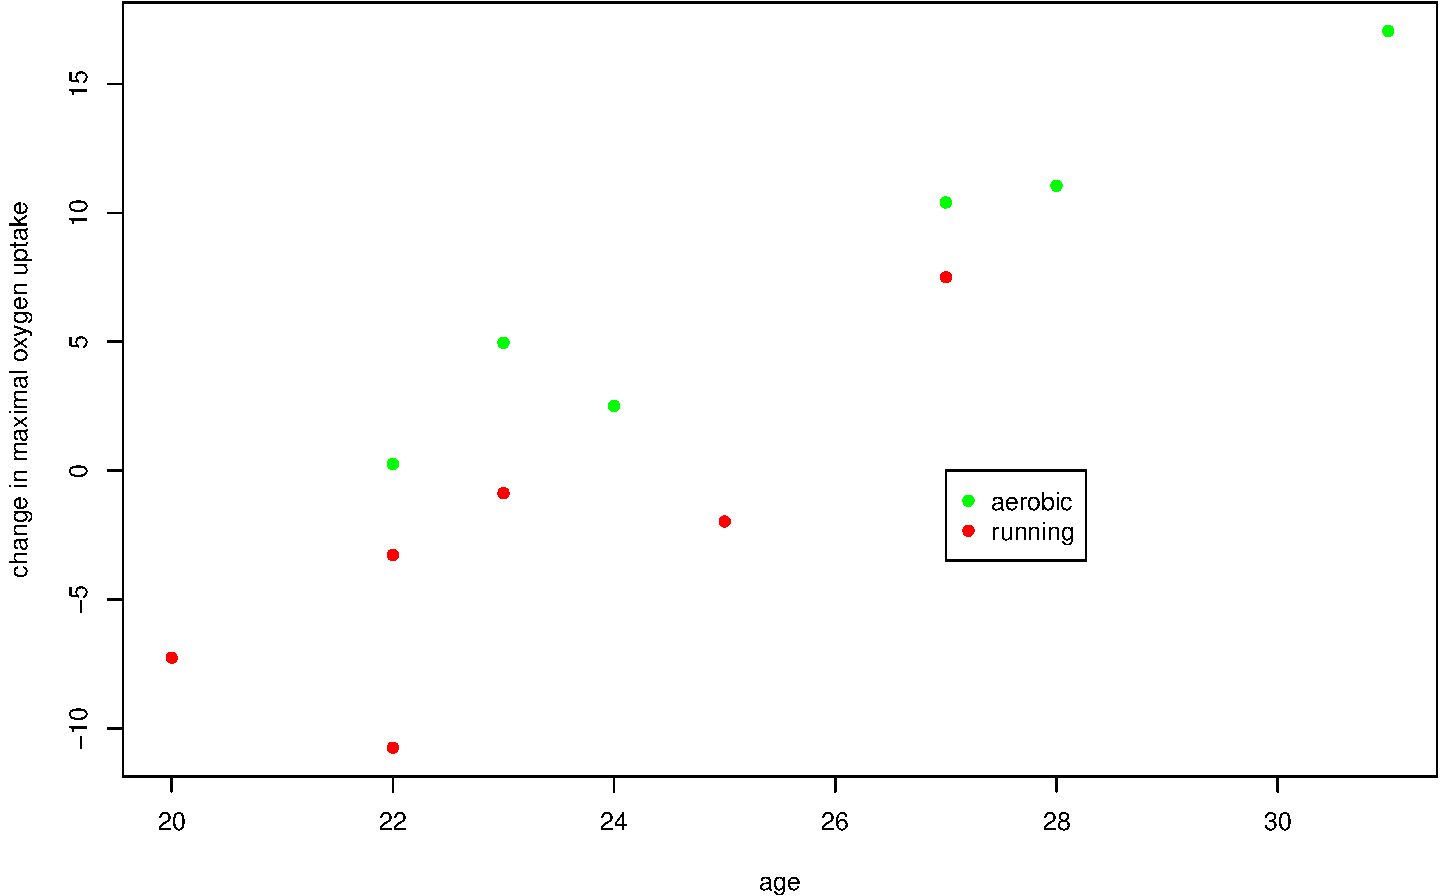
\includegraphics{9-linear-regression_files/figure-beamer/unnamed-chunk-2-1.pdf}

\end{frame}

\begin{frame}{Data analysis}
\protect\hypertarget{data-analysis}{}

\(y\) = change in oxygen uptake (scalar)

\(x_1\) = exercise indicator (0 for running, 1 for aerobic)

\(x_2\) = age

How can we estimate \(p(y \mid x_1, x_2)?\)

\end{frame}

\begin{frame}{Linear regression}
\protect\hypertarget{linear-regression}{}

Assume that smoothness is a function of age.

For each group,

\[y = \beta_o + \beta_1 x_2 + \epsilon\]

Linearity means \textbf{linear in the parameters} (\(\beta\)'s).

\end{frame}

\begin{frame}{Linear regression}
\protect\hypertarget{linear-regression-1}{}

We could also try the model

\[y = \beta_o + \beta_1 x_2 +  \beta_2 x_2^2 + \beta_3 x_2^3 + \epsilon\]

which is also a linear regression model.

\end{frame}

\begin{frame}{Notation}
\protect\hypertarget{notation}{}

\begin{itemize}
\tightlist
\item
  \(X_{n\times p}\): regression features or covariates (design matrix)
\item
  \(\bx_i\): \(i\)th row vector of the regression covariates
\item
  \(\by_{n\times 1}\): response variable (vector)
\item
  \(\bbeta_{p \times 1}\): vector of regression coefficients
\end{itemize}

\end{frame}

\begin{frame}{Notation (continued)}
\protect\hypertarget{notation-continued}{}

\[\bm{X}_{n \times p} = 
\left( \begin{array}{cccc}
x_{11} & x_{12} & \ldots&  x_{1p}\\
x_{21} & x_{22} & \ldots& x_{2p} \\
x_{i1} & x_{i2} & \ldots& x_{ip} \\
\vdots & \vdots & \ddots & \vdots \\
x_{n1} & x_{n2} &\ldots& x_{np}
\end{array} \right).
\]

\begin{itemize}
\item
  A column of x represents a particular covariate we might be interested
  in, such as age of a person.
\item
  Denote \(x_i\) as the ith \textcolor{red}{row vector} of the
  \(X_{n \times p}\) matrix.
\end{itemize}

\[  x_{i}= \left( \begin{array}{c}
x_{i1}\\
\textcolor{red}{x_{i2}}\\
\vdots\\
x_{ip}
\end{array} \right) \]

\end{frame}

\begin{frame}{Notation (continued)}
\protect\hypertarget{notation-continued-1}{}

\[  \bbeta= \left( \begin{array}{c}
\beta_1\\
\beta_2\\
\vdots\\
\beta_p
\end{array} \right) \]

\[  \by= \left( \begin{array}{c}
y_1\\
y_2\\
\vdots\\
y_n
\end{array} \right) \]

\[\by_{n \times 1} = 
X_{n \times p} \bbeta_{p \times 1} + \bm{\epsilon}_{n \times 1}\]

\end{frame}

\begin{frame}{Regression models}
\protect\hypertarget{regression-models}{}

How does an outcome \(\bm{y}\) vary as a function of the covariates
which we represent as \(X_{n\times p}\) matrix?

\begin{itemize}
\tightlist
\item
  Can we predict \(\bm{y}\) as a function of each row in the matrix
  \(X_{n\times p}\) denoted by \(\bx_i.\)
\item
  Which \(\bx_i\)'s have an effect?
\end{itemize}

Such questions can be assessed via a linear regression model
\(p(\by \mid X).\)

\end{frame}

\begin{frame}{Multiple linear regression}
\protect\hypertarget{multiple-linear-regression}{}

Consider the following:

\[y_i = \beta_1 x_{i1} + \beta_2 x_{i2} + \beta_3 x_{i3} + 
\beta_4 x_{i4} + \epsilon_i\]

where \begin{align}
x_{i1} &= 1 \; \text{for subject} \; i \\
x_{i2} &= 0 \; \text{for running}; \text{1 for aerobics}  \\
x_{i3} &= \text{age of subject i}\\
x_{i4} &= x_{i2} \times x_{i3} 
\end{align}

Under this model,
\[E[\bm{y} \mid \bm{x}] = \beta_1 + \beta_3 \times age \; \text{if} \; x_2=0\]
\[E[\bm{y} \mid \bm{x}] = (\beta_1 + \beta_2) + (\beta_3 + \beta_4)\times age \; \text{if} \; x_2=1 \]

\end{frame}

\begin{frame}{Least squares regression lines}
\protect\hypertarget{least-squares-regression-lines}{}

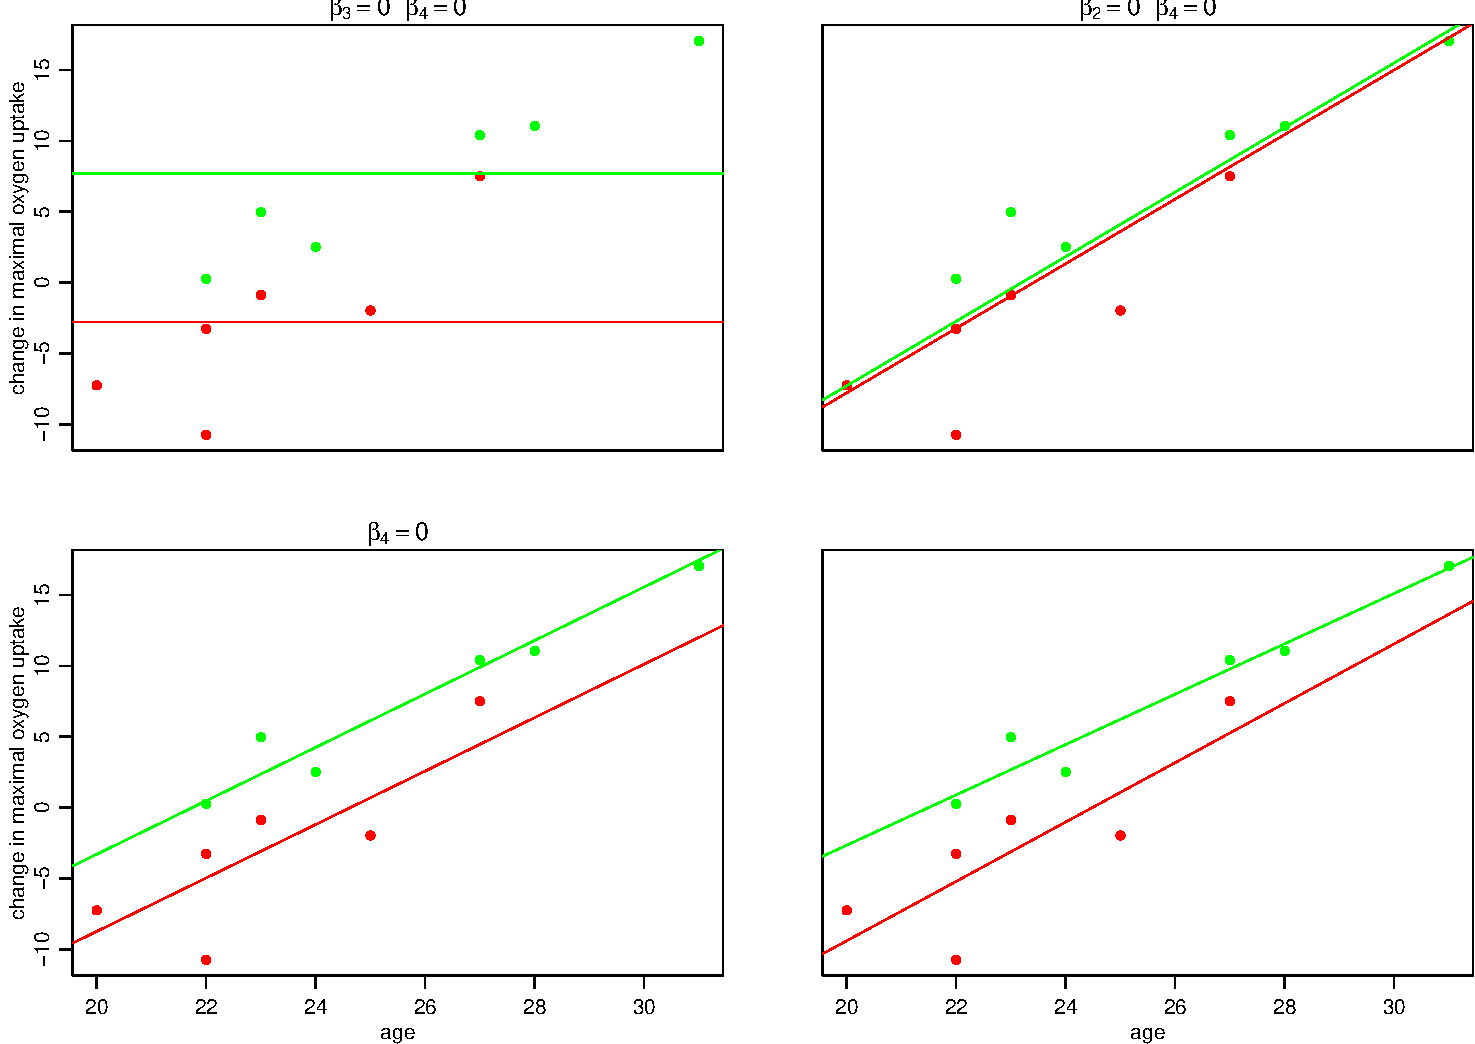
\includegraphics{9-linear-regression_files/figure-beamer/unnamed-chunk-3-1.pdf}

\end{frame}

\begin{frame}{Multivariate Setup}
\protect\hypertarget{multivariate-setup}{}

Let's assume that we have data points \((x_i, y_i)\) available for all
\(i=1,\ldots,n.\)

\begin{itemize}
\item
  \(y\) is the response variable \[  \by= \left( \begin{array}{c}
  y_1\\
  y_2\\
  \vdots\\
  y_n
  \end{array} \right)_{n \times 1} \]
\item
  \(\bx_{i}\) is the \(i\)th row of the design matrix
  \(X_{n \times p}.\)
\end{itemize}

Consider the regression coefficients

\[  \bbeta = \left( \begin{array}{c}
\beta_{1}\\
\beta_{2}\\
\vdots\\
\beta_{p}
\end{array} \right)_{p \times 1} \]

\end{frame}

\begin{frame}{Normal Regression Model}
\protect\hypertarget{normal-regression-model}{}

The Normal regression model specifies that

\begin{itemize}
\tightlist
\item
  \(E[Y\mid \bx_i]\) is linear and
\item
  the sampling variability around the mean is independently and
  identically (iid) drawn from a normal distribution
\end{itemize}

\begin{align}
Y_i &= \bbeta^T \bx_i + \bm{\epsilon}_i\\
\epsilon_1,\ldots,\epsilon_n &\stackrel{iid}{\sim} \text{Normal}(0,\sigma^2)
\end{align}

This implies
\(Y_i \mid \bbeta, \bx_i \sim \text{Normal}(\bbeta^T \bx_i,\sigma^2).\)

\end{frame}

\begin{frame}{Multivariate Bayesian Normal Regression Model}
\protect\hypertarget{multivariate-bayesian-normal-regression-model}{}

We can re-write this as a multivariate regression model as:

\[\by \mid X,\bbeta, \sigma^2 \sim \text{MVN}( X\bbeta, \sigma^2 I_p).\]

We can specify a multivariate Bayesian model as:

\[\by \mid X,\bbeta, \sigma^2 \sim \text{MVN}( X\bbeta, \sigma^2 I_p)\]
\[\bbeta \sim \text{MVN}(0, \tau^2 I_p),\]

where \(\sigma^2, \tau^2\) are known.

\end{frame}

\begin{frame}{Bayesian Normal Regression Model}
\protect\hypertarget{bayesian-normal-regression-model}{}

The likelihood is \begin{align}
&p(y_1,\ldots,y_n \mid x_1,\ldots x_n, \bbeta, \sigma^2) \\
&= \prod_{i=1}^n p(\by_i \mid \bx_i, \bbeta, \sigma^2) \\
&(2\pi \sigma^2 )^{-n/2} \exp\{
\frac{-1}{2\sigma^2} \sum_{i=1}^n (\by_i - \bbeta^T \bx_i)^2
\}\\
&= (2\pi \sigma^2 )^{-n/2} \exp\{\textcolor{black}{-\frac{1}{2}} (\by - X\bbeta)^T\textcolor{black}{(\sigma^2)^{-1} I_p}(\by - X\bbeta)\}
\end{align}

\end{frame}

\begin{frame}{Background}
\protect\hypertarget{background}{}

The Euclidean norm (\(L^2\) norm or square root of the sum of squares)
of \(\boldsymbol{y} = (y_1, \ldots, y_n)\) is defined by

\[ \|\boldsymbol{y}\|_2 = \sqrt{y_1^2 + \ldots + y_n^2}.\] It follows
that

\[ \|\boldsymbol{y}\|_2^2 = y_1^2 + \ldots + y_n^2.\] \vspace*{1em}

\textbf{Why do we use this notation?} It's compact and convenient!

\end{frame}

\begin{frame}{Background}
\protect\hypertarget{background-1}{}

We would like to find \[\argmin_{\bbeta \in \R^p} \|\by-X\bbeta\|_2^2,\]

where the \(\argmin\) (the arguments of the minima) are the points or
elements of the domains of some function as which the functions values
are minimized.

\end{frame}

\begin{frame}{Ordinary Least Squares}
\protect\hypertarget{ordinary-least-squares}{}

We can estimate the coefficients \(\hat{\bm{\beta}} \in \R^p\) by least
squares:
\[\hat{\bm{\beta}} = \argmin_{\bbeta \in \R^p} \|\by-X\bbeta\|_2^2\]

One can show that \[\hat{\bm{\beta}} = (X^T X)^{-1} X^T \by\]

\bigskip

The fitted values are
\[\textcolor{black}{\hat{\bm{y}}} = X\hat{\bm{\beta}} = X(X^T X)^{-1} X^T \by\]
This is a linear function of \(\by\), \(\hy = H\by\), where
\(H=X(X^T X)^{-1} X^T\) is sometimes called the \textbf{hat matrix}.

\end{frame}

\begin{frame}{Exercise 1 (OLS)}
\protect\hypertarget{exercise-1-ols}{}

Let SSR denote sum of squared residuals.
\[ \min_{\bbeta} SSR(\bbeta) = \min_{\bbeta} \|\by-X{\bm{\beta}}\|_2^2\]
Show that \[\hat{\bm{\beta}}  = (X^TX)^{-1}X^T\by.\]

\end{frame}

\begin{frame}{Ordinary Least squares estimation}
\protect\hypertarget{ordinary-least-squares-estimation}{}

Proof: Observe \begin{align}
 \frac{\partial SSR(\bbeta)}{\partial \bbeta} 
 &:=  \frac{\partial \|\by-X{\bm{\beta}}\|_2^2}{\partial \bbeta} \\
&= \frac{\partial (\by-X\bbeta)^T(\by-X\bbeta)}{\partial \bbeta} \\
&= \frac{\partial \by^T\by - 2\bbeta^TX^T\by + \hbeta^T(X^TX)\bbeta}{\partial \bbeta}\\
& = -  2X^T\by + 2X^TX\bbeta
\end{align}

This implies
\(-X^T\by + X^TX\bbeta= 0 \implies \hat{\bm{\beta}}_{ols} = (X^TX)^{-1}X^T\by.\)
\vskip 1em

This is called the \textbf{ordinary least squares estimator}. How do we
know it is unique?

\end{frame}

\begin{frame}{Exercise 2 (OLS)}
\protect\hypertarget{exercise-2-ols}{}

Show that

\[\hat{\bm{\beta}} \sim MVN(\bbeta, \sigma^2  (X^TX)^{-1}).\]

\end{frame}

\begin{frame}{Ordinary Least squares estimation}
\protect\hypertarget{ordinary-least-squares-estimation-1}{}

Proof: Recall

\[\hbeta  = (X^TX)^{-1}X^T\bY. \] \vskip 1em
\[E(\hat{\bm{\beta}} ) = E[(X^TX)^{-1}X^T\bY]= 
(X^TX)^{-1}X^T E[\bY] = (X^TX)^{-1}X^TX
\bbeta.\]

\vskip 1em \begin{align}
\Var(\hat{\bm{\beta}}) &= \Var\{ (X^TX)^{-1}X^T\bY\}\\
 &=
(X^TX)^{-1}X^T \sigma^2 I_n X (X^TX)^{-1}\\
& = \sigma^2  (X^TX)^{-1}
\end{align}

\[\hat{\bm{\beta}} \sim MVN(\bbeta, \sigma^2  (X^TX)^{-1}).\]

\end{frame}

\begin{frame}[fragile]{Recall data set up}
\protect\hypertarget{recall-data-set-up}{}

\footnotesize

\begin{Shaded}
\begin{Highlighting}[]
\CommentTok{# running is 0, 1 is aerobic}
\NormalTok{x1<-}\KeywordTok{c}\NormalTok{(}\DecValTok{0}\NormalTok{,}\DecValTok{0}\NormalTok{,}\DecValTok{0}\NormalTok{,}\DecValTok{0}\NormalTok{,}\DecValTok{0}\NormalTok{,}\DecValTok{0}\NormalTok{,}\DecValTok{1}\NormalTok{,}\DecValTok{1}\NormalTok{,}\DecValTok{1}\NormalTok{,}\DecValTok{1}\NormalTok{,}\DecValTok{1}\NormalTok{,}\DecValTok{1}\NormalTok{)}
\CommentTok{# age}
\NormalTok{x2<-}\KeywordTok{c}\NormalTok{(}\DecValTok{23}\NormalTok{,}\DecValTok{22}\NormalTok{,}\DecValTok{22}\NormalTok{,}\DecValTok{25}\NormalTok{,}\DecValTok{27}\NormalTok{,}\DecValTok{20}\NormalTok{,}\DecValTok{31}\NormalTok{,}\DecValTok{23}\NormalTok{,}\DecValTok{27}\NormalTok{,}\DecValTok{28}\NormalTok{,}\DecValTok{22}\NormalTok{,}\DecValTok{24}\NormalTok{)}
\CommentTok{# change in maximal oxygen uptake}
\NormalTok{y<-}\KeywordTok{c}\NormalTok{(}\OperatorTok{-}\FloatTok{0.87}\NormalTok{,}\OperatorTok{-}\FloatTok{10.74}\NormalTok{,}\OperatorTok{-}\FloatTok{3.27}\NormalTok{,}\OperatorTok{-}\FloatTok{1.97}\NormalTok{,}\FloatTok{7.50}\NormalTok{,}
     \FloatTok{-7.25}\NormalTok{,}\FloatTok{17.05}\NormalTok{,}\FloatTok{4.96}\NormalTok{,}\FloatTok{10.40}\NormalTok{,}\FloatTok{11.05}\NormalTok{,}\FloatTok{0.26}\NormalTok{,}\FloatTok{2.51}\NormalTok{)}
\end{Highlighting}
\end{Shaded}

\end{frame}

\begin{frame}[fragile]{Recall data set up}
\protect\hypertarget{recall-data-set-up-1}{}

\footnotesize

\begin{Shaded}
\begin{Highlighting}[]
\NormalTok{(x3 <-}\StringTok{ }\NormalTok{x2) }\CommentTok{#age}
\end{Highlighting}
\end{Shaded}

\begin{verbatim}
##  [1] 23 22 22 25 27 20 31 23 27 28 22 24
\end{verbatim}

\begin{Shaded}
\begin{Highlighting}[]
\NormalTok{(x2 <-}\StringTok{ }\NormalTok{x1) }\CommentTok{#aerobic versus running }
\end{Highlighting}
\end{Shaded}

\begin{verbatim}
##  [1] 0 0 0 0 0 0 1 1 1 1 1 1
\end{verbatim}

\begin{Shaded}
\begin{Highlighting}[]
\NormalTok{(x1<-}\StringTok{ }\KeywordTok{seq}\NormalTok{(}\DecValTok{1}\OperatorTok{:}\KeywordTok{length}\NormalTok{(x2))) }\CommentTok{#index of person}
\end{Highlighting}
\end{Shaded}

\begin{verbatim}
##  [1]  1  2  3  4  5  6  7  8  9 10 11 12
\end{verbatim}

\begin{Shaded}
\begin{Highlighting}[]
\NormalTok{(x4 <-}\StringTok{ }\NormalTok{x2}\OperatorTok{*}\NormalTok{x3)}
\end{Highlighting}
\end{Shaded}

\begin{verbatim}
##  [1]  0  0  0  0  0  0 31 23 27 28 22 24
\end{verbatim}

\end{frame}

\begin{frame}[fragile]{Recall data set up}
\protect\hypertarget{recall-data-set-up-2}{}

\footnotesize

\begin{Shaded}
\begin{Highlighting}[]
\NormalTok{(X <-}\StringTok{ }\KeywordTok{cbind}\NormalTok{(x1,x2,x3,x4))}
\end{Highlighting}
\end{Shaded}

\begin{verbatim}
##       x1 x2 x3 x4
##  [1,]  1  0 23  0
##  [2,]  2  0 22  0
##  [3,]  3  0 22  0
##  [4,]  4  0 25  0
##  [5,]  5  0 27  0
##  [6,]  6  0 20  0
##  [7,]  7  1 31 31
##  [8,]  8  1 23 23
##  [9,]  9  1 27 27
## [10,] 10  1 28 28
## [11,] 11  1 22 22
## [12,] 12  1 24 24
\end{verbatim}

\end{frame}

\begin{frame}[fragile]{OLS estimation in R}
\protect\hypertarget{ols-estimation-in-r}{}

\footnotesize

\begin{Shaded}
\begin{Highlighting}[]
\CommentTok{## using the lm function}
\NormalTok{fit.ols<-}\KeywordTok{lm}\NormalTok{(y}\OperatorTok{~}\StringTok{ }\NormalTok{X[,}\DecValTok{2}\NormalTok{] }\OperatorTok{+}\StringTok{ }\NormalTok{X[,}\DecValTok{3}\NormalTok{] }\OperatorTok{+}\NormalTok{X[,}\DecValTok{4}\NormalTok{])}
\KeywordTok{summary}\NormalTok{(fit.ols)}\OperatorTok{$}\NormalTok{coef}
\end{Highlighting}
\end{Shaded}

\begin{verbatim}
##                Estimate Std. Error    t value    Pr(>|t|)
## (Intercept) -51.2939459 12.2522126 -4.1865047 0.003052321
## X[, 2]       13.1070904 15.7619762  0.8315639 0.429775106
## X[, 3]        2.0947027  0.5263585  3.9796120 0.004063901
## X[, 4]       -0.3182438  0.6498086 -0.4897500 0.637457484
\end{verbatim}

\end{frame}

\begin{frame}{Exercise 3 (Multivariate inference for regression models)}
\protect\hypertarget{exercise-3-multivariate-inference-for-regression-models}{}

Let \begin{align}
\bm{y} &\mid \bbeta \sim \text{MVN}(X \bbeta, \sigma^2 I)\\
\bbeta &\sim \text{MVN}(\bbeta_0, \Sigma_0)
\end{align}

Show that the posterior is
\[\bbeta \mid \bm{y}, X \sim \text{MVN}(\bbeta_n, \Sigma_n), \; \text{where}\]
\begin{align*}
\bbeta_n &= E[\bbeta\ \mid \bm{y}, \bX, \sigma^2] = (\Sigma_o^{-1} + (nX^TX)/\sigma^2)^{-1}
(\Sigma_o^{-1}\bbeta_0 + \bX^T\bm{\bar{y}}/\sigma^2) \\
\Sigma_n &= \text{Var}[\bbeta \mid \bm{y}, X, \sigma^2] = (\Sigma_o^{-1} + (nX^TX)/\sigma^2)^{-1}
\end{align*}

Remark: If \(\Sigma_o^{-1} << (X^TX)^{-1}\) then
\(\bbeta_n \approx \hat{\bbeta}_{ols}\)

If \(\Sigma_o^{-1} >> (X^TX)^{-1}\) then \(\bbeta_n \approx \bbeta_{0}\)

\end{frame}

\begin{frame}{Exercise 3 Solution}
\protect\hypertarget{exercise-3-solution}{}

Let's start with the likelihood: \begin{align}
\bm{y} &\mid \bbeta \sim \text{MVN}(X \bbeta, \sigma^2 I)
\end{align}

\begin{align}
p(\bm{y}  \mid  \bbeta) &\propto \exp\{\frac{-1}{2\sigma^2}
\sum_{i=1}^n
(\bm{y}_i - X\bbeta)^T(\bm{y}_i - X\bbeta)
\} \\
&\propto \exp\{\frac{-1}{2\sigma^2}
\sum_{i=1}^n
[
\bm{y}_i^T\bm{y}_i + \bbeta^TX^TX\bbeta - 2\bbeta^TX^T\bm{y}_i
]
\}\\
&\propto \exp\{\frac{-1}{2\sigma^2}
\sum_{i=1}^n
[
\bbeta^TX^TX\bbeta - 2\bbeta^TX^T\bm{y}_i
]
\}\\
&\propto \exp\{-\frac{1}{2}
[
\bbeta^T\textcolor{blue}{\frac{n\;X^TX}{\sigma^2}}\bbeta - 2\bbeta^T\textcolor{red}{\frac{X^T\bar{\bm{y}}}{\sigma^2}}
]
\}
\end{align}

This implies that \(A_1 = \frac{n\;X^TX}{\sigma^2}\) and
\(b_1 = \frac{X^T\bar{\bm{y}}}{\sigma^2}.\)

\end{frame}

\begin{frame}{Exercise 3 Solution}
\protect\hypertarget{exercise-3-solution-1}{}

Now, let's consider the prior.

\begin{align}
\bbeta &\sim \text{MVN}(\bbeta_0, \Sigma_0)
\end{align}

\begin{align}
p(\bbeta) 
&\propto \exp\{-\frac{1}{2}
(\bbeta - \bbeta_0)^T\Sigma_0^{-1}(\bbeta - \bbeta_0)
\} \\
&\propto \exp\{-\frac{1}{2}
[\bbeta^T \Sigma_0^{-1} \bbeta +\bbeta_0^T\Sigma_0^{-1}\bbeta_0 - 2 \bbeta^T\Sigma_0^{-1}\bbeta_0]
\} \\
&\propto \exp\{-\frac{1}{2}
[\bbeta^T \textcolor{blue}{\Sigma_0^{-1}} \bbeta - 2 \bbeta^T\textcolor{red}{\Sigma_0^{-1}\bbeta_0}]
\} 
\end{align}

This implies that \(A_o = \Sigma_0^{-1}\) and
\(b_o = \Sigma_0^{-1}\bbeta_0.\)

\end{frame}

\begin{frame}{Exercise 3 Solution}
\protect\hypertarget{exercise-3-solution-2}{}

The posterior is

\begin{align}
p(\bbeta \mid \bm{y}) &\propto
\exp\{-\frac{1}{2}
[
\bbeta^T\textcolor{blue}{\frac{n\;X^TX}{\sigma^2}}\bbeta - 2\bbeta^T\textcolor{red}{\frac{X^T\bar{\bm{y}}}{\sigma^2}}
]
\}\\
&\times
\exp\{-\frac{1}{2}
[\bbeta^T \textcolor{blue}{\Sigma_0^{-1}} \bbeta - 2 \bbeta^T\textcolor{red}{\Sigma_0^{-1}\bbeta_0}]
\} \\
&= \exp\{-\frac{1}{2}
[
\bbeta^T \textcolor{blue}{A_1} \bbeta - 2\bbeta^T \textcolor{red}{b_1}
]
\}\\
&\times \qquad \exp\{-\frac{1}{2}
[
\bbeta^T \textcolor{blue}{A_o} \bbeta - 2\bbeta^T \textcolor{red}{b_o}
]
\} \\
&= \exp\{-\frac{1}{2}
[
\bbeta^T \textcolor{blue}{(A_o + A_1)} \bbeta - 2\bbeta^T \textcolor{red}{(b_o + b_1)}
]
\}
\end{align}

\end{frame}

\begin{frame}{Exercise 3 Solution}
\protect\hypertarget{exercise-3-solution-3}{}

Let \(A_n = A_o + A_1\) and \(b_n = b_o + b_1.\)

Using the kernel of the multivariate normal, we can now find the
posterior mean and the posterior covariance:

\[A_n = A_o + A_1 = \Sigma_0^{-1} + \frac{n\;X^TX}{\sigma^2}.\]
\[b_n = b_o + b_1 = \Sigma_0^{-1}\bbeta_0 + \frac{X^T\bar{\bm{y}}}{\sigma^2}.\]
\[\bbeta \mid \bm{y} \sim MVN(A_n^{-1} b_n, A_n^{-1}) =: MVN(\bbeta_n, \Sigma_n),\]

where
\[\mu_n = (\Sigma_0^{-1} + \frac{n\;X^TX}{\sigma^2})^{-1}(\Sigma_0^{-1}\bbeta_0 + \frac{X^T\bar{\bm{y}}}{\sigma^2})\]
and

\[\Sigma_n = (\Sigma_0^{-1} + \frac{n\;X^TX}{\sigma^2})^{-1}.\]

\end{frame}

\begin{frame}{Multivariate inference for regression models}
\protect\hypertarget{multivariate-inference-for-regression-models}{}

The posterior from Exercise 3 can be shown to be
\[\bbeta \mid \bm{y}, X \sim \text{MVN}(\bbeta_n, \Sigma_n)\]

where

\[\bbeta_n = E[\bbeta\ \mid \bm{y}, \bX, \sigma^2] = (\Sigma_o^{-1} + (nX^TX)/\sigma^2)^{-1}
(\Sigma_o^{-1}\bbeta_0 + X^T\bm{y}/\sigma^2)\]

\[\Sigma_n = \text{Var}[\bbeta \mid \bm{y}, \bX, \sigma^2] = (\Sigma_o^{-1} + (nX^TX)/\sigma^2)^{-1}\]

\end{frame}

\begin{frame}{Setting prior parameters}
\protect\hypertarget{setting-prior-parameters}{}

How would you set the prior parameters for

\begin{itemize}
\tightlist
\item
  \(\sigma^2\)
\item
  \(\Sigma_{o}\)
\item
  \(\beta_0\)
\end{itemize}

\end{frame}

\begin{frame}{Setting prior parameters}
\protect\hypertarget{setting-prior-parameters-1}{}

\begin{itemize}
\item
  Estimate \(\sigma^2\) by
  \(\dfrac{y^Ty - \hat{\beta}_{ols}^TX^Ty}{n - (p + 1)}\) because this
  is an unbiased estimator of \(\sigma^2.\)
\item
  Set \[\Sigma_{o}^{-1} = \frac{(X^TX)}{n\sigma^2},\] which is known as
  the unit information prior (Kass and Wasserman, 1995).
\item
  Set \(\beta_0 = \hat{\beta}_{ols}.\) (This centers the prior
  distribution of \(\beta\) around the OLS estimate).
\end{itemize}

\textbf{Why are these reasonable choices?}

\end{frame}

\begin{frame}{Setting prior parameters}
\protect\hypertarget{setting-prior-parameters-2}{}

\begin{itemize}
\item
  Do you think that the posterior would be sensitive to the choice of
  these parameters?
\item
  How could you improve upon our choices regarding priors on \(\beta_0\)
  and \(\Sigma_0\)?
\end{itemize}

\end{frame}

\begin{frame}{The g-prior}
\protect\hypertarget{the-g-prior}{}

To improve things by doing the \textbf{least amount of calculus}, we can
put a \emph{g-prior} on \(\bbeta\) (not \(\bbeta_0).\)

The g-prior on \(\bbeta\) has the following form:
\[ \bbeta \mid \bX, \sigma^2  \sim MVN(0, g\; \sigma^2 (\bX^T\bX)^{-1}),\]
where \(g\) is a constant, such as \(g=n.\)

It can be shown that (Zellner, 1986):

\begin{enumerate}
\tightlist
\item
  g shrinks the coefficients and can prevent overfitting to the data
\item
  if \(g = n\), then as n increases, inference approximates that using
  \(\hat{\beta}_{ols}\)
\end{enumerate}

\end{frame}

\begin{frame}{The g-prior}
\protect\hypertarget{the-g-prior-1}{}

Under the g-prior, it follows that \begin{align}
\bbeta_n &= E[\bbeta\ \mid \bm{y}, \bX, \sigma^2]  \\
&= \left(\frac{X^TX}{g \sigma^2} + \frac{X^TX}{\sigma^2}\right)^{-1} \frac{X^Ty}{\sigma^2} \\
&= \frac{g}{g+1} (X^TX)^{-1} X^Ty
= \frac{g}{g+1} \hat{\beta}_{ols}
\end{align}

\begin{align}
\Sigma_n &= \text{Var}[\bbeta \mid \bm{y}, \bX, \sigma^2] \\
&= \left(\frac{X^TX}{g \sigma^2} + \frac{X^TX}{\sigma^2}\right)^{-1}
=\frac{g}{g+1} \sigma^2 (X^TX)^{-1} \\
&= \frac{g}{g+1} \Var[\hat{\beta}_{ols}]
\end{align}

\end{frame}

\begin{frame}{Prior on \(\Sigma_0\)}
\protect\hypertarget{prior-on-sigma_0}{}

What prior would you place on \(\Sigma_0\) and why?

\end{frame}

\begin{frame}{Next steps}
\protect\hypertarget{next-steps}{}

\begin{itemize}
\item
  How do all these concepts fit together? How can you build a
  hierarhical model using linear regression and the tools that you've
  learned?
\item
  I recommend doing the derivations from this module on your own.
\item
  I recommend reading through Hoff to solidify you knowledge. This
  material is around page 153, but chapter 9 is helpful regarding being
  complementary to this material.
\item
  You could also code this up to further solidify you knowledge of this,
  but you'll get practice on this with lab 10 and homework 8.
\end{itemize}

\end{frame}

\begin{frame}{Linear Regression Applied to Swimming (Lab 10)}
\protect\hypertarget{linear-regression-applied-to-swimming-lab-10}{}

\begin{itemize}
\tightlist
\item
  We will consider Exercise 9.1 in Hoff very closely to illustrate
  linear regression.
\item
  The data set we consider contains times (in seconds) of four high
  school swimmers swimming 50 yards.
\item
  There are 6 times for each student, taken every two weeks.
\item
  Each row corresponds to a swimmer and a higher column index indicates
  a later date.
\item
  This corresponds with Lab 10 and Homework 8 (the last homework)!
\end{itemize}

\end{frame}

\begin{frame}[fragile]{Data set}
\protect\hypertarget{data-set}{}

\begin{Shaded}
\begin{Highlighting}[]
\KeywordTok{read.table}\NormalTok{(}\StringTok{"data/swim.dat"}\NormalTok{,}\DataTypeTok{header=}\OtherTok{FALSE}\NormalTok{)}
\end{Highlighting}
\end{Shaded}

\begin{verbatim}
## Warning in read.table("data/swim.dat", header = FALSE): incomplete final line
## found by readTableHeader on 'data/swim.dat'
\end{verbatim}

\begin{verbatim}
##     V1   V2   V3   V4   V5   V6
## 1 23.1 23.2 22.9 22.9 22.8 22.7
## 2 23.2 23.1 23.4 23.5 23.5 23.4
## 3 22.7 22.6 22.8 22.8 22.9 22.8
## 4 23.7 23.6 23.7 23.5 23.5 23.4
\end{verbatim}

\end{frame}

\begin{frame}{Full conditionals (Task 1)}
\protect\hypertarget{full-conditionals-task-1}{}

We will fit a separate linear regression model for each swimmer, with
swimming time as the response and week as the explanatory variable. Let
\(y_{i}\in \mathbbm{R}^{6}\) be the 6 recorded times for swimmer \(i.\)
Let \[X_i =
\begin{bmatrix}
    1 & 1  \\
    1 & 3 \\ 
    ... \\
    1 & 9\\
    1 & 11
\end{bmatrix}
\] be the design matrix for swimmer \(i.\) Then we use the following
linear regression model: \begin{align*}
    Y_i &\sim \mathcal{N}_6\left(X_i\beta_i, \tau_i^{-1}\mathcal{I}_6\right) \\
    \beta_i &\sim \mathcal{N}_2\left(\beta_0, \Sigma_0\right) \\
    \tau_i &\sim \text{Gamma}(a,b).
\end{align*} Derive full conditionals for \(\beta_i\) and \(\tau_i.\)

\end{frame}

\begin{frame}{Solution (Task 1)}
\protect\hypertarget{solution-task-1}{}

The conditional posterior for \(\beta_i\) is multivariate normal with
\begin{align*}
    \mathbbm{V}[\beta_i \, | \, Y_i, X_i, \textcolor{red}{\tau_i} ] &= (\Sigma_0^{-1} + \textcolor{red}{\tau_i} X_i^{T}X_i)^{-1}\\ 
    \mathbbm{E}[\beta_i \, | \, Y_i, X_i, \textcolor{red}{\tau_i} ] &= 
    (\Sigma_0^{-1} + \textcolor{red}{\tau_i} X_i^{T}X_i)^{-1} (\Sigma_0^{-1}\beta_0 + \textcolor{red}{\tau_i} X_i^{T}Y_i).
\end{align*} while \begin{align*}
    \tau_i \, | \, Y_i, X_i, \beta &\sim \text{Gamma}\left(a + 3\, , \, b + \frac{(Y_i - X_i\beta_i)^{T}(Y_i - X_i\beta_i)}{2} \right).
\end{align*}

These can be found in in Hoff in section 9.2.1.

\textbf{I highly recommend that you derive these as practice for the final exam.}

\end{frame}

\begin{frame}{Task 2}
\protect\hypertarget{task-2}{}

Complete the prior specification by choosing \(a,b,\beta_0,\) and
\(\Sigma_0.\) Let your choices be informed by the fact that times for
this age group tend to be between 22 and 24 seconds.

\end{frame}

\begin{frame}{Solution (Task 2)}
\protect\hypertarget{solution-task-2}{}

Choose \(a=b=0.1\) so as to be somewhat uninformative.

Choose \(\beta_0 = [23\,\,\, 0]^{T}\) with \[\Sigma_0 =
\begin{bmatrix}
    5 & 0  \\
    0 & 2 
\end{bmatrix}.
\] This centers the intercept at 23 (the middle of the given range) and
the slope at 0 (so we are assuming no increase) but we choose the
variance to be a bit large to err on the side of being less informative.

\end{frame}

\begin{frame}{Gibbs sampler (Task 3)}
\protect\hypertarget{gibbs-sampler-task-3}{}

Code a Gibbs sampler to fit each of the models. For each swimmer \(i,\)
obtain draws from the posterior predictive distribution for \(y_i^{*},\)
the time of swimmer \(i\) if they were to swim two weeks from the last
recorded time.

\end{frame}

\begin{frame}{Posterior Prediction (Task 4)}
\protect\hypertarget{posterior-prediction-task-4}{}

The coach has to decide which swimmer should compete in a meet two weeks
from the last recorded time. Using the posterior predictive
distributions, compute
\(\text{Pr}\left\{y_i^{*}=\text{max}\left(y_1^{*},y_2^{*},y_3^{*},y_4^{*}\right)\right\}\)
for each swimmer \(i\) and use these probabilities to make a
recommendation to the coach.

\end{frame}

\begin{frame}{Final Grades}
\protect\hypertarget{final-grades}{}

I am proposing to drop your lowest exam grade (out of Exam I, Exam II,
and the Final Exam).

\begin{itemize}
\item
  Homework: 30 percent
\item
  Highest Exam: 35
\item
  Second Highest Exam: 35
\item
  So your \textbf{two highest exam scores} will be weighted evenly and
  you lowest exam score will be completely dropped.
\item
  Yes, you still must take the final exam.
\end{itemize}

\end{frame}

\begin{frame}{Course Evaluations}
\protect\hypertarget{course-evaluations}{}

\begin{itemize}
\tightlist
\item
  I would be very appreciative if you would fill out the course
  evaluations
\item
  They are located on DukeHub
\item
  Directions:
  \url{https://assessment.trinity.duke.edu/students-course-evaluations}
\item
  If there is a 100 percent response rate, I will give everyone in the
  course 1 point on their final exam grade.
\end{itemize}

\end{frame}

\begin{frame}{Exam II}
\protect\hypertarget{exam-ii}{}

\begin{itemize}
\tightlist
\item
  Students did extremely well on problems 1 and 2.
\item
  You should feel very proud of how you did on these problems. Great
  job!
\end{itemize}

\end{frame}

\begin{frame}{Exam II}
\protect\hypertarget{exam-ii-1}{}

There were issues on both problems 3 and 4.

Due to this, I'm releasing Exam II:
\url{https://github.com/resteorts/modern-bayes/blob/master/exercises/final-exam/exam2-2020-version2.pdf}

No solutions will be posted to encourage you to work through these
derivations on your own. See a member of the TA Team if you have a
question, and make sure to bring your derivation with you so we can help
understand how best to help you!

\end{frame}

\end{document}
